\documentclass[border=10pt]{standalone}
\usepackage[svgnames]{xcolor}
\usepackage{amsmath}
\usepackage{pgfplots}
\pgfplotsset{compat=newest}
\usepackage[sfdefault]{FiraSans}
\usepackage{FiraMono}
\renewcommand*\familydefault{\sfdefault}
\begin{document}
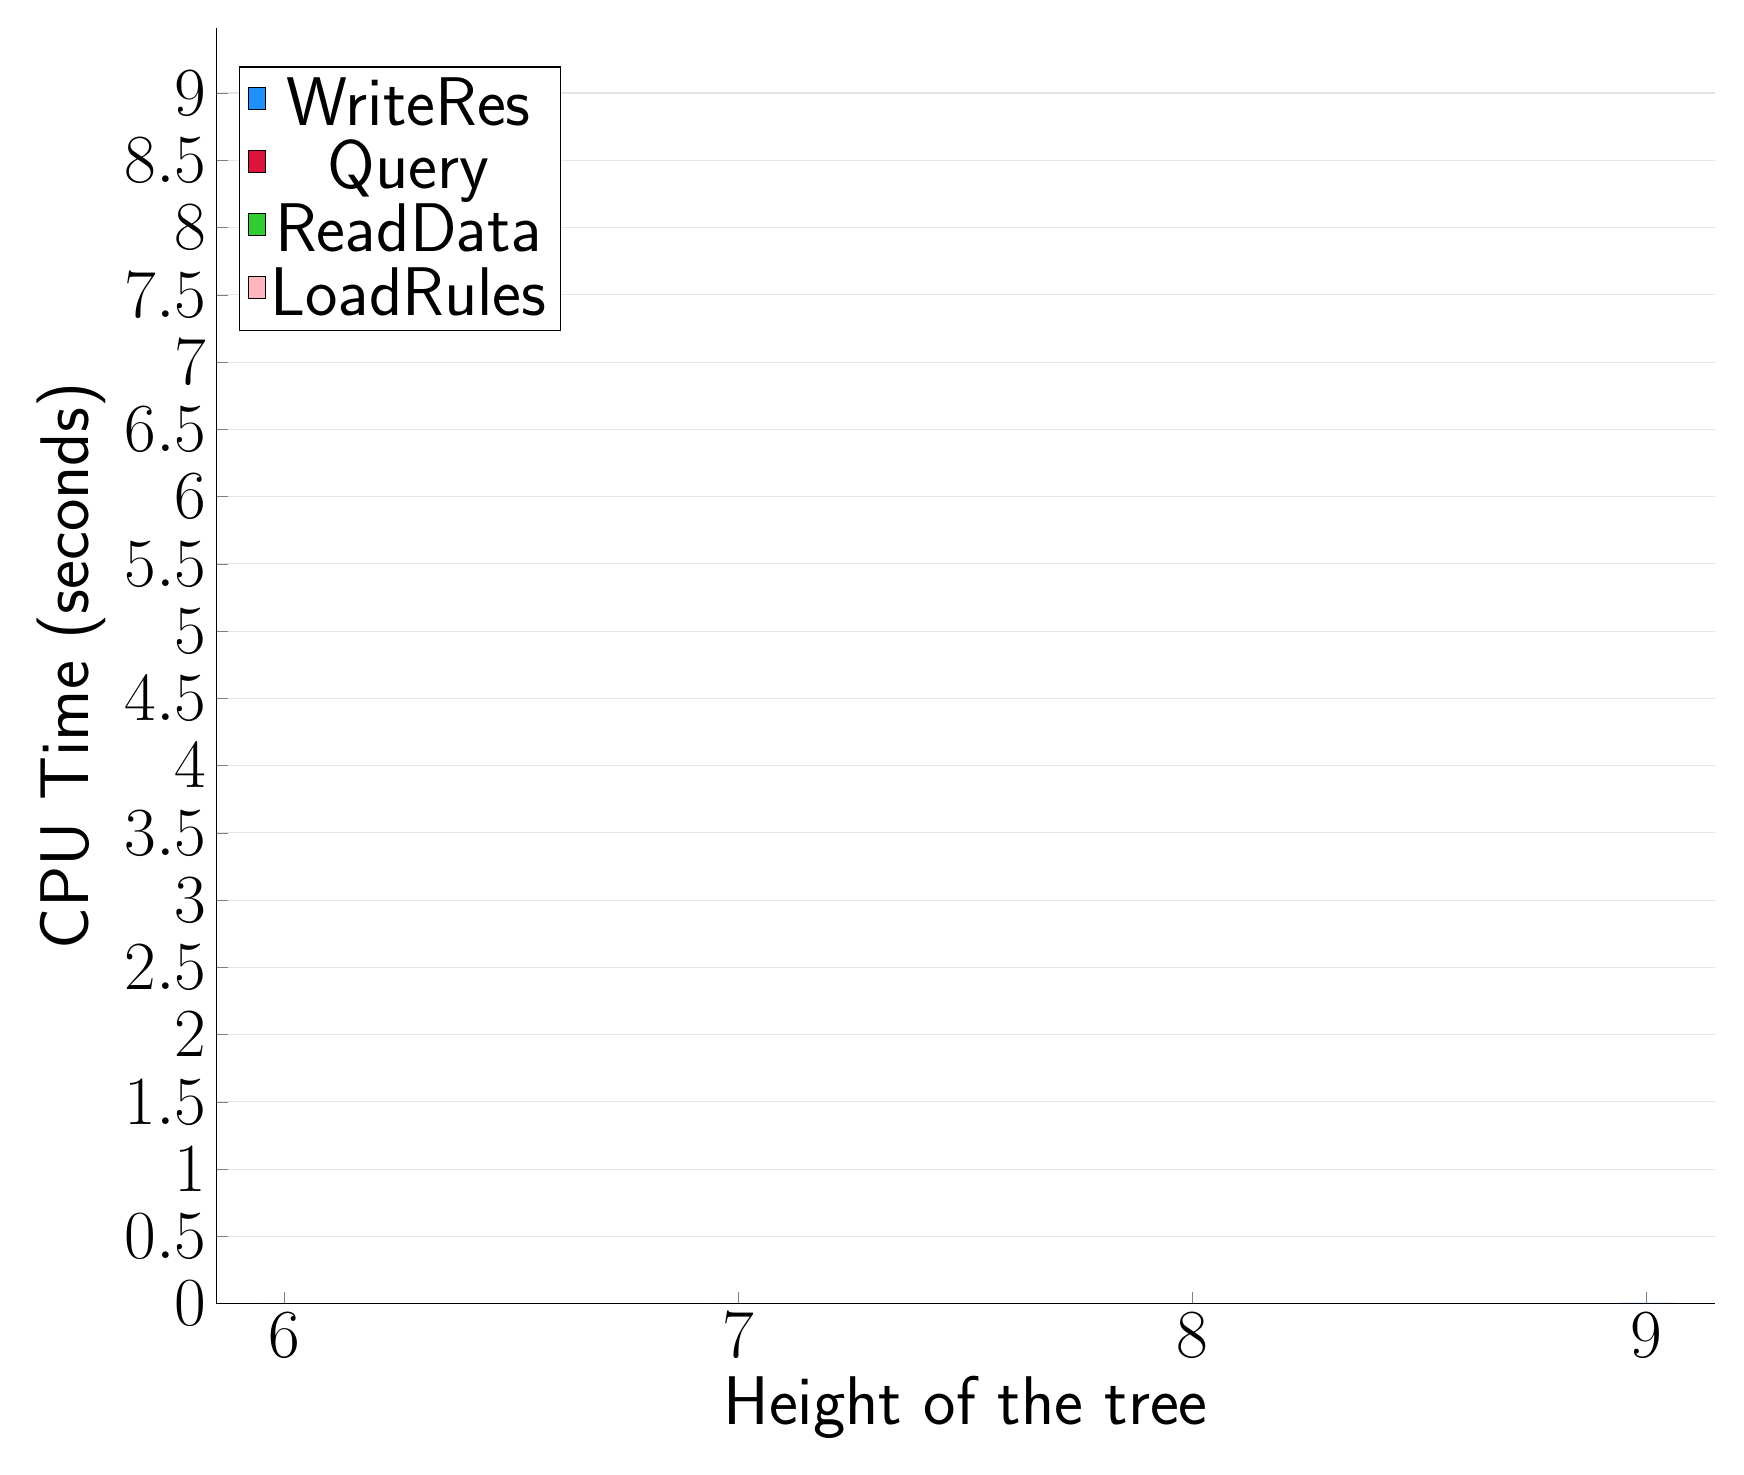
\begin{tikzpicture}
\begin{axis}[
   ybar stacked,
   width=1.7\textwidth,
   bar width=0.7cm,
   ymajorgrids, tick align=inside,
   major grid style={draw=gray!20},
   xtick=data,
   ymin=0, ymax=9.482,
   axis x line*=bottom,
   axis y line*=left,
   enlarge x limits=0.05,
   legend style={
       at={(0.23, 0.97)},
       anchor=north east,
       legend columns=1,
       font=\Huge,
   },
   ylabel={CPU Time (seconds)},
   xlabel={Height of the tree},
   label style={font=\Huge},
   tick label style={font=\Huge},
]
\addlegendimage{fill=DodgerBlue, draw=black, line width=0.2pt}
\addlegendentry{WriteRes}
\addlegendimage{fill=Crimson, draw=black, line width=0.2pt}
\addlegendentry{Query}
\addlegendimage{fill=LimeGreen, draw=black, line width=0.2pt}
\addlegendentry{ReadData}
\addlegendimage{fill=LightPink, draw=black, line width=0.2pt}
\addlegendentry{LoadRules}
\addplot +[fill=LightPink, draw=black, line width=0.2pt] coordinates {
(6, 0.0005489999999999994)
(7, 0.0005481999999999998)
(8, 0.0005491999999999999)
(8, 0.0005521999999999994)
(8, 0.0005474)
(9, 0.0005504)
(9, 0.0005468)
(9, 0.0005444)
(9, 0.0005514000000000004)
(9, 0.0005479999999999998)
};
\addplot +[fill=LimeGreen, draw=black, line width=0.2pt] coordinates {
(6, 0.0001702000000000004)
(7, 0.000218)
(8, 0.0003160000000000004)
(8, 0.0003159999999999998)
(8, 0.0003151999999999998)
(9, 0.0005187999999999998)
(9, 0.0005176000000000002)
(9, 0.0005165999999999999)
(9, 0.0005173999999999997)
(9, 0.0005172000000000006)
};
\addplot +[fill=Crimson, draw=black, line width=0.2pt] coordinates {
(6, 7.319999999999998e-05)
(7, 0.000178)
(8, 0.0004408)
(8, 0.00044139999999999994)
(8, 0.0004406000000000002)
(9, 0.0011022)
(9, 0.0011102)
(9, 0.0011014)
(9, 0.0011042)
(9, 0.0011094)
};
\addplot +[fill=DodgerBlue, draw=black, line width=0.2pt] coordinates {
(6, 0.0002775999999999998)
(7, 0.0006190000000000002)
(8, 0.001363)
(8, 0.0013694000000000002)
(8, 0.0013507999999999999)
(9, 0.003048)
(9, 0.0030800000000000003)
(9, 0.0030352)
(9, 0.0030732)
(9, 0.0030514)
};
\end{axis}
\end{tikzpicture}

\end{document}
